\chapter{Conclusions and Final Remarks}
\label{chap:conclusions}

This work discusses how to combine wearable computing, edge computing, and AI to define a new field of knowledge where these formerly antagonist methods can be employed together, namely Wearable Edge AI. Then, we use this new field to create new wearable technologies based on this concept. Thus, our main objective with this work is to establish a Wearable Edge AI concept and define how to design and create applications in this context. 

With this text, we expect to understand how to create cooperative wearable systems based on edge computing, considering real-time aspects. We also review the HW/SW co-design process to evaluate architectural aspects. Finally, we performed a series of case studies to evaluate aspects of the risen concepts and methods.

Wearable computing, which has a central role in this work, is a concept that arose in the late 90s and early 2000s. In modern approaches, these applications use hardware miniaturization and the IoT to increase the number of possible applications within this perspective. Edge computing is another concept that uses the IoT to develop and rise. It comes to solving issues that cloud computing struggles with, such as real-time and low latency. This concept happens using proximity as a factor and in perspectives that provide the services with powerful computing, emulate the cloud services, or enhance the processing limits on mobile appliances. AI is a general concept of machines that can learn to solve real-world problems. More recently, ML applications have been pushed toward the clouds, given their requirement for high computational power.

Although wearable and edge computing have requirements that diverge from AI, an increasing number of authors are trying to combine these concepts to create novel solutions. This uprising trend still needed to have a general definition. Our case studies are some examples of how the proposed solutions seek to mesh the concepts of machine learning and edge computing.

To establish the Wearable Edge AI concept, we started with the grounding knowledge in edge computing and machine learning. Then, we defined Edge AI as the set of methods that describes the design process and validation of solutions that combine edge computing and machine learning concepts to develop novel appliances, systems, and applications to solve real-world problems. Finally, we proposed a taxonomy method to classify Edge AI applications. The works are initially classified according to their edge computing paradigm (cloudlets, fog computing, or mobile edge computing) and then through an AI classification that divides them into ``machine learning'' and ``deep learning'' applications. 

We continued by defining Edge AI and evaluating the concepts behind cooperative wearable systems. Then, we evaluated the design process to consider novel constraints based on the added edge computing process. Finally, we defined Wearable Edge AI as the set of methods that describes the design process and validation of solutions that combine wearable computing and Edge AI concepts in developing novel appliances, systems, and applications to solve real-world problems.

\section{Theoretical Backbone}

\begin{figure}[h!]
    \centering
    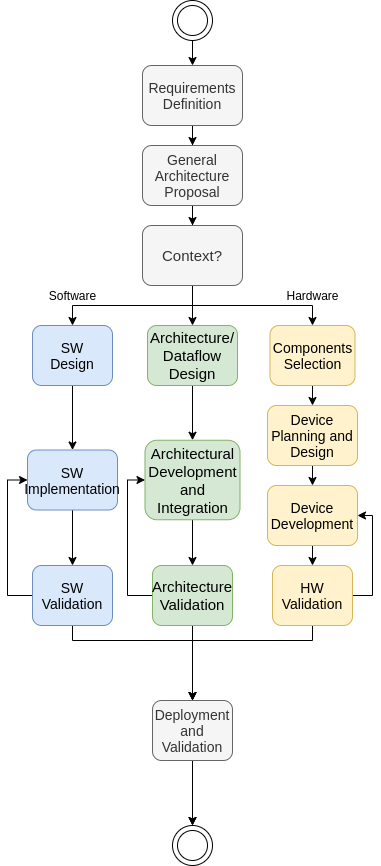
\includegraphics[width = .37\linewidth]{Figures/codesign-2.0.png}
    \caption{New co-design approach}
    \label{fig:codesign-conclusion}
\end{figure}

Our design process definition is centered on the redefinition of the classical hardware/software co-design process. This concept comes from the development of embedded systems but required some updates to consider edge computing traits. Figure \ref{fig:codesign-conclusion} displays the result of our evaluation.

This approach provided the means to propose solutions within the Wearable Edge AI concept for the two stakeholders from this work. Our experiments display strong evidence that this update provides a valuable tool for developing new solutions combining the concepts of Edge Computing, Wearable Computing, and AI. In all cases, we display how some of the constraints do not fit well within the hardware or software constraints, being specifically analyzed as architectural traits. Each application had a gain in evaluating the architectural traits in parallel with the hardware and software design:

\begin{itemize}
	\item \textbf{Leaf damage estimation:} In this case, the architectural traits helped selecting the AI framework to develop the application. This appliance must be feasible to run in embedded hardware with accelerated AI, as it has the most computationally consuming algorithm within this context.
	\item \textbf{Evaluating and mapping diseases in forest canopies:} This application requires the concepts of cooperative wearable systems as a baseline to work. Integrating the wearable solutions within an Edge Server requires an evaluation under the optic of architectural restraints.
	\item \textbf{Ant distribution and counting estimation:} In this work, the algorithm design and backbone choices considered a constrained wearable edge AI environment. The model has a smaller memory footprint, with the feasibility of running in embedded edge servers.
	\item \textbf{Physical condition monitoring in field:} This application uses the cooperative wearable systems baseline to provide information for a multidisciplinary team. In this case, an understanding of the architecture is essential to designing an application and understanding its limits.
	\item \textbf{Smart wearable systems in the context of COVID-19:} This application design integrates several wearable devices within a local wireless network environment. Therefore, the proposal and results depend on the definition of architectural restrictions.
	\item \textbf{Wearable-based human activity recognition:} This application is another example of using multiple wearable devices within an interconnected edge computing architecture. Therefore, its capabilities also depend on the establishment of architectural restrictions.
\end{itemize}

\section{Lessons learned}

In this work, we explored a set of case studies in which the concepts of Wearable Edge AI apply. We have identified a set of lessons learned along this work. These lessons come from the conceptualization of Edge AI up to the application development. They are:

\begin{itemize}
	\item \textbf{Wearable Edge AI requires Mobile Edge AI.} The constraints observed in developing Wearable Edge AI applications are similar to those of Mobile Edge AI. Nevertheless, these restrictions are increased by the nature of the applications.
	\item \textbf{Wearable Edge AI applications required a review of the Hardware/Software co-design.} The original co-design process described how to create embedded applications but was not enough to consider the integration of cooperative devices within a network. Thus, this concept required a revision to design Edge AI applications.
	\item \textbf{Wearable Edge AI adds further constraints related to the architecture.} As its foundation is the Internet of Things (IoT), considering machine-to-machine communication, these applications have another set of constraints considering the architecture and machine-to-machine communication.
	\item \textbf{AI and computer vision usually add computationally constrained methods into Wearable Edge AI systems.} Timing is an essential constraint within Wearable Edge AI. Algorithms must have performance and avoid consuming too much computing resources during their functioning. Therefore, costly algorithms such as image processing and AI profoundly impact the applications' performance. 
	\item \textbf{Hardware, Software, and Architectural constraints often are complementary.} Some constraints come from hardware requirements but will be surpassed by software decisions. A typical example in our cases was an edge server's processing and energetic constraint, which directly impacts the hardware choice and architecture design. Therefore, the branches of the co-design cannot be interpreted as isolated development stages.
\end{itemize}

\section{Future Works}

In future works, we suggest using this set of rules to create a Wearable Edge AI development framework. This step consolidates the concepts raised within this text into a set of tools to develop novel cyber-physical applications. Also, we encourage other researchers to create more applications within the context of the presented stakeholders, as we displayed some of their needs within this text.